\section{Развёртывание, эксплуатация и экспериментальная проверка}

\subsection{Стенд и контур проверки}

Экспериментальная проверка выполнялась на контейнерном стенде, разворачиваемом через Docker Compose. В состав стенда входили прикладные сервисы notification-facade, template-registry, profile-consent, scheduler-delivery, notification-mail-sender, notification-sms-sender и history-writer, а также Kafka, отдельные PostgreSQL-хранилища операционных сервисов, MongoDB, Redis, ClickHouse, Prometheus и Grafana.

Такой стенд воспроизводит не только набор сервисов, но и границы хранения, поэтому подходит для проверки маршрута целиком: gRPC-команда, запись события, Kafka-публикация, sender-обработка и запись результата в аналитическую историю доставки.

Стенд запускался локально на рабочей станции под управлением Windows 10 с процессором класса Intel Core i7 13-го поколения и 16~ГБ оперативной памяти. Это важно для интерпретации результатов: проверка проводилась не на выделенном сервере, а в ограниченном локальном окружении, где контейнеры приложений, брокер, базы данных и средства наблюдаемости конкурировали за одни и те же ресурсы хоста.

Ключевые параметры нагрузочного стенда и генератора приведены в таблице~\ref{tab:load-stand-config}. В основной части оставлены только те настройки, которые влияют на интерпретацию маршрута и масштаба нагрузки.

\begin{table}[H]
    \centering
    \footnotesize
    \renewcommand{\arraystretch}{1.15}
    \caption{Конфигурация нагрузочного стенда}
    \label{tab:load-stand-config}
    \begin{tabular}{|L{0.34\textwidth}|L{0.50\textwidth}|}
        \hline
        \textbf{Параметр} & \textbf{Значение} \\
        \hline
        Платформа хоста & Windows 10, локальный запуск в Docker Compose \\
        \hline
        Аппаратная конфигурация & процессор класса Intel Core i7 13-го поколения, 16 ГБ RAM \\
        \hline
        Число уникальных пользователей & 10000 подготовленных получателей \\
        \hline
        Число потоков генератора & 10 \\
        \hline
        Профиль входной нагрузки & линейный разгон от 25 до 90 запросов в секунду \\
        \hline
        Длительность активной фазы & 1800 секунд \\
        \hline
        Получателей в одном запросе & случайное число от 2 до 10 \\
        \hline
    \end{tabular}
\end{table}

\subsection{Методика проверки}

Нагрузочный прогон использовался для двух задач: проверки связности полного маршрута обработки и получения базовых количественных характеристик стенда. Целью не было определение предельной промышленной производительности, однако полученные значения RPS и задержек позволяют оценить поведение системы под устойчивой нагрузкой.

Проверка выполнялась в четыре этапа:
\begin{enumerate}
    \item подготовка стенда и приведение хранилищ к контролируемому начальному состоянию;
    \item выполнение функциональных и сквозных сценариев;
    \item серия из трёх повторных нагрузочных прогонов через custom-loader после предварительного заполнения Redis-профилей;
    \item сбор и интерпретация метрик gRPC, Kafka и JVM по артефактам Grafana.
\end{enumerate}

До серии нагрузочных прогонов выполнялись подготовительный seed получателей и ручная проверка базовых сценариев: создание события, немедленный запуск, отложенный запуск, email-доставка, SMS-доставка и запись итогового статуса в history-writer. Повторные прогоны выполнялись с одним и тем же профилем нагрузки; в тексте ниже приводятся усреднённые значения и характерные диапазоны порядка величин, а не псевдоточные цифры до единиц сообщений.

\subsection{Критерии успешности}

Критерии успешности нагрузочного прогона приведены в таблице~\ref{tab:test-success-criteria}.

\begin{table}[H]
    \centering
    \footnotesize
    \renewcommand{\arraystretch}{1.15}
    \caption{Критерии успешности нагрузочного прогона}
    \label{tab:test-success-criteria}
    \begin{tabular}{|L{0.27\textwidth}|L{0.29\textwidth}|L{0.30\textwidth}|}
        \hline
        \textbf{Критерий} & \textbf{Ожидаемый результат} & \textbf{Фактический результат} \\
        \hline
        Входной gRPC-контур принимает команды & Метрика CreateNotificationEvent имеет ненулевой поток запросов в активной фазе & Ненулевой поток подтверждён графиком server RPS; медианная задержка CreateNotificationEvent составила около 786 ms \\
        \hline
        События передаются в Kafka & Producer и listener metrics фиксируют публикацию и потребление сообщений & Для notification.facade.events среднее потребление составило 38.3 сообщения в секунду, максимум 47.3 сообщения в секунду \\
        \hline
        Sender-сервисы потребляют события & Канальные listener-метрики имеют ненулевой поток и конечное время обработки & Среднее listener-время mail-sender составило 47.2 ms, для scheduler-delivery --- 41--58 ms в сценарии отложенного запуска \\
        \hline
        Статусы доходят до history-writer & delivery-statuses потребляются и сохраняются & Среднее потребление notification.delivery-statuses составило 21.5 сообщения в секунду, среднее listener-время history-writer --- 46.9 ms \\
        \hline
        Система остаётся наблюдаемой & Доступны gRPC, Kafka и JVM-метрики по всем ключевым участкам маршрута & Маршрут восстанавливается по Grafana-артефактам server RPS, gRPC latency, Kafka publish latency и Kafka consume RPS \\
        \hline
    \end{tabular}
\end{table}

\subsection{Проверка механизмов повторной обработки}

Таблица~\ref{tab:repeat-processing-checks} отделяет заявленные механизмы repeat-processing от общей нагрузки и показывает, какие сценарии были подтверждены на стенде, а какие требуют отдельной дополнительной фиксации.

\begin{table}[H]
    \centering
    \footnotesize
    \renewcommand{\arraystretch}{1.15}
    \caption{Проверка механизмов повторной обработки}
    \label{tab:repeat-processing-checks}
    \begin{tabular}{|L{0.26\textwidth}|L{0.19\textwidth}|L{0.22\textwidth}|L{0.23\textwidth}|}
        \hline
        \textbf{Сценарий} & \textbf{Проверяемый механизм} & \textbf{Ожидаемый результат} & \textbf{Фактический результат} \\
        \hline
        Повторный CreateNotificationEvent с тем же idempotency key & idempotency key, unique constraint & Новое уведомительное событие не создаётся & TODO: требуется зафиксировать отдельный протокол повторного вызова и ответ фасада в артефактах стенда \\
        \hline
        Повторное получение Kafka-сообщения sender-сервисом & transactional inbox, deduplication & Доставка не создаётся повторно & Сценарий заложен в модель consumer inbox и уникальных ограничений; в текущем наборе выгрузок отдельный счётчик подавленных дублей отсутствует \\
        \hline
        Временная ошибка внешнего провайдера & retry policy & Доставка переводится в повторную попытку или в контролируемую ошибку & TODO: требуется сохранить отдельный лог или метрику по retry для mail- и sms-контуров \\
        \hline
        Недоступность profile-consent при канальной обработке & ошибка профильной проверки, статусная фиксация & Сообщение не теряется; результат фиксируется статусом или повторной попыткой & Проверен отказозависимый маршрут через обязательный вызов profile-consent; отдельная статистика по forced-failure в текущем прогоне не сохранялась \\
        \hline
        Запись итогового статуса в history-writer & status event, Kafka, history storage & Изменение статуса появляется в истории & Подтверждено потреблением notification.delivery-statuses и записью итогового статуса в history-writer \\
        \hline
    \end{tabular}
\end{table}

\subsection{Проверенные сценарии}

На стенде были подтверждены следующие сценарии:
\begin{enumerate}
    \item создание уведомительного события и фиксация аудитории;
    \item немедленный запуск доставки;
    \item отложенный запуск через scheduler-delivery;
    \item обработка email- и SMS-запусков как двух независимых канальных контуров;
    \item проверка профиля получателя перед отправкой;
    \item запись итогового статуса в history-writer;
    \item повторная обработка входящего сообщения без неконтролируемого дубля.
\end{enumerate}

Функциональная проверка показала, что полный маршрут не распадается на несвязанные фрагменты: событие, запуск, канальная доставка и история проходят через разные сервисные границы, но сохраняют идентифицируемую связь.

\subsection{Артефакты метрик}

Для анализа использовались четыре группы метрик:
\begin{enumerate}
    \item gRPC server metrics для notification-facade, profile-consent и history-writer;
    \item Kafka producer metrics для публикации событий и статусных сообщений;
    \item Kafka listener metrics для sender-сервисов и history-writer;
    \item JVM/process metrics как эксплуатационный фон.
\end{enumerate}

\begin{figure}[H]
    \centering
    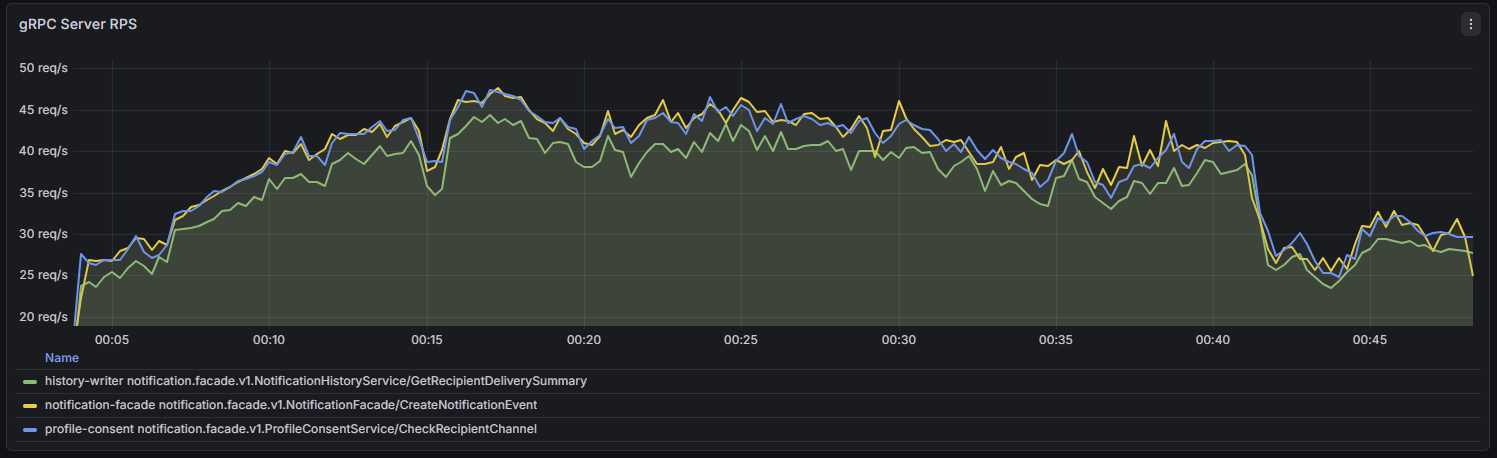
\includegraphics[width=\textwidth]{inc/server_rps.png}
    \caption{Интенсивность gRPC-вызовов в ходе нагрузочного прогона}
    \label{fig:test-server-rps}
\end{figure}

Рисунок~\ref{fig:test-server-rps} используется как временная шкала активной фазы прогона. По нему видно, что CreateNotificationEvent, CheckRecipientChannel и GetRecipientDeliverySummary наблюдаются как независимые сервисные вызовы, а не как один монолитный маршрут. Для архитектуры это подтверждает разделение ролей между фасадом, profile-consent и history-writer.

\begin{figure}[H]
    \centering
    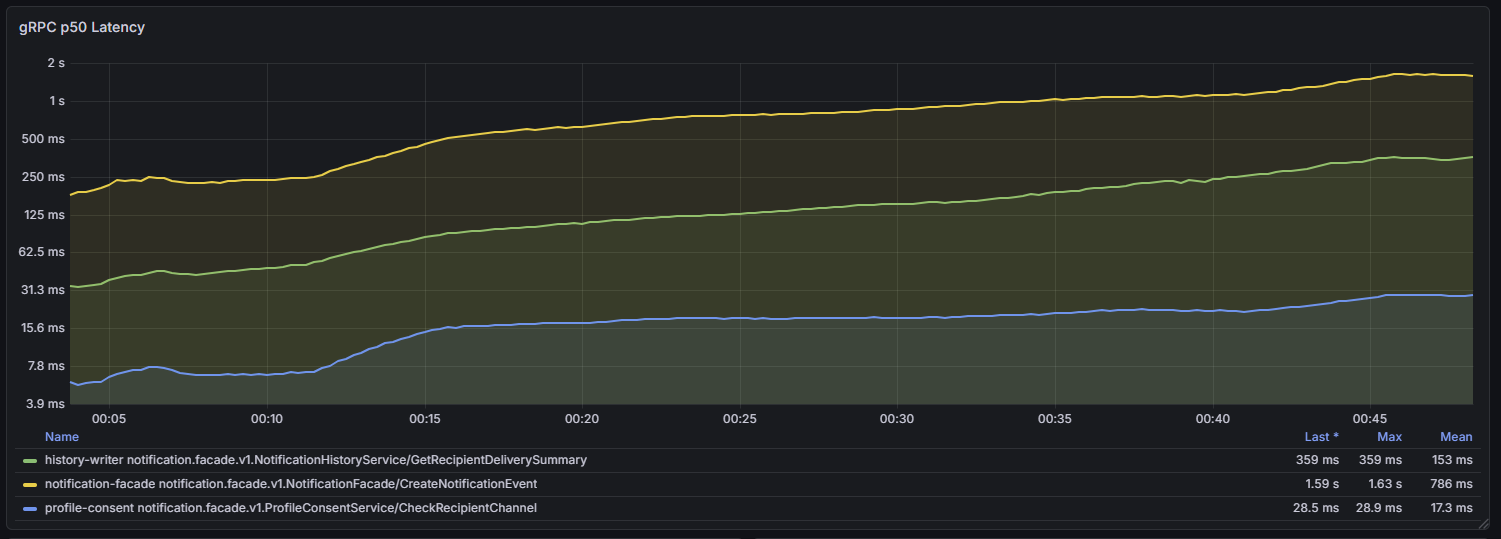
\includegraphics[width=\textwidth]{inc/grpc_p50_lat.png}
    \caption{Медианная задержка gRPC-вызовов}
    \label{fig:test-grpc-p50}
\end{figure}

Рисунок~\ref{fig:test-grpc-p50} показывает, что самый тяжёлый синхронный вызов в наблюдаемом наборе --- CreateNotificationEvent. Это ожидаемо: именно на этом этапе выполняются валидация запроса, запись события и подготовка публикации в Kafka. При этом задержки profile-consent и history-writer остаются существенно ниже, что подтверждает их роль как поддерживающих сервисов, а не доминирующих узких мест командного контура.

\begin{figure}[H]
    \centering
    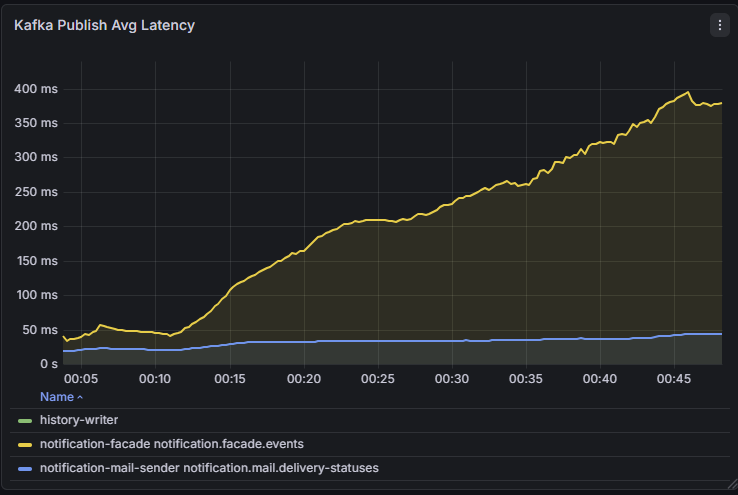
\includegraphics[width=\textwidth]{inc/kafka_avg_latency.png}
    \caption{Средняя задержка публикации Kafka-сообщений}
    \label{fig:test-kafka-publish-latency}
\end{figure}

Рисунок~\ref{fig:test-kafka-publish-latency} нужен для оценки стоимости перехода из синхронного контура в асинхронный. Рост средней задержки публикации для notification.facade.events показывает, что брокер и producer-участок дают заметный вклад в суммарное время маршрута. Одновременно график остаётся ограниченным сверху и не показывает признаков необратимого накопления деградации.

\begin{figure}[H]
    \centering
    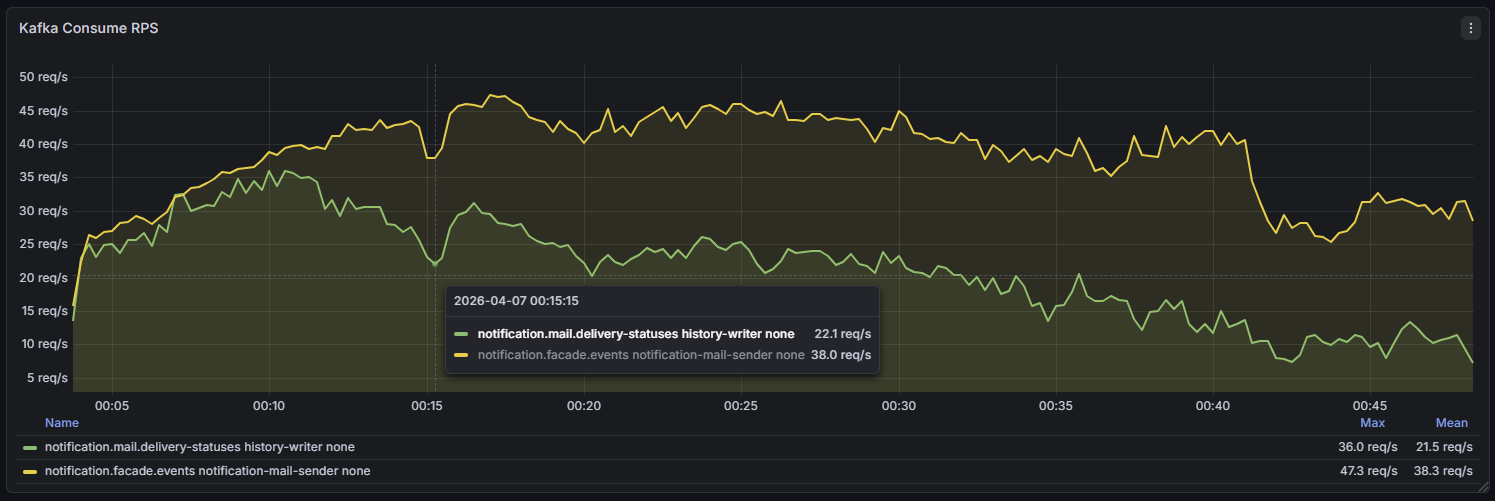
\includegraphics[width=\textwidth]{inc/kafka_consume_rps.png}
    \caption{Интенсивность потребления Kafka-сообщений}
    \label{fig:test-kafka-consume-rps}
\end{figure}

Рисунок~\ref{fig:test-kafka-consume-rps} подтверждает прохождение маршрута до конечной стадии. На нём одновременно видны потребление notification.facade.events канальным обработчиком и потребление notification.delivery-statuses сервисом history-writer. Это означает, что нагрузочный прогон затрагивает не только входной фасад и публикацию в Kafka, но и завершение жизненного цикла уведомления.

\subsection{Результаты нагрузочного прогона}

Итоговые показатели серии прогонов приведены в таблицах~\ref{tab:load-results-volume} и~\ref{tab:load-results-latency}. Числа даны как усреднённые ориентиры и диапазоны по трём повторным прогонам с одинаковой конфигурацией генератора нагрузки. Отдельно учитывались сценарии немедленного и отложенного запуска доставки.

\begin{table}[H]
    \centering
    \footnotesize
    \renewcommand{\arraystretch}{1.15}
    \caption{Параметры прогона и маршрутные показатели}
    \label{tab:load-results-volume}
    \begin{tabular}{|L{0.32\textwidth}|L{0.22\textwidth}|L{0.36\textwidth}|}
        \hline
        \textbf{Показатель} & \textbf{Значение} & \textbf{Интерпретация} \\
        \hline
        Число прогонов & 3 & повторение профиля использовалось для проверки устойчивости порядка величин \\
        \hline
        Активная фаза прогона & 43--45 минут & период наблюдения по временной шкале Grafana для каждого прогона \\
        \hline
        Подготовленных получателей & 10000 & исходная аудитория, подготовленная seed-этапом \\
        \hline
        Профиль входной нагрузки & 25 $\rightarrow$ 90 req/s, 1800 c & линейный разгон нагрузки в основном командном контуре \\
        \hline
        Событий за прогон & порядка 95--105 тыс. & оценка по профилю генератора и наблюдаемому темпу командного контура \\
        \hline
        Запусков доставки за прогон & порядка 95--105 тыс. & немедленный запуск следует за созданием события без дополнительного синхронного ожидания \\
        \hline
        notification.facade.events consume & mean 38.3 req/s, max 47.3 req/s & подтверждает стабильную работу входа в канальный контур \\
        \hline
        Статусных событий за прогон & порядка 54--58 тыс. & оценка по среднему потреблению статусного топика и длительности активной фазы \\
        \hline
        notification.delivery-statuses consume & mean 21.5 req/s, max 36.0 req/s & подтверждает прохождение маршрута до конечной статусной стадии \\
        \hline
        Отложенных запусков за прогон & порядка 18--25 тыс. & отдельный сценарий с публикацией через scheduled-контур \\
        \hline
        notification.mail.scheduled consume & mean 19--24 req/s, max 31--34 req/s & показывает, что планировщик удерживает и затем переводит запуск в рабочий канал \\
        \hline
    \end{tabular}
\end{table}

\begin{table}[H]
    \centering
    \footnotesize
    \renewcommand{\arraystretch}{1.15}
    \caption{Задержки gRPC- и Kafka-контуров}
    \label{tab:load-results-latency}
    \begin{tabular}{|L{0.32\textwidth}|L{0.22\textwidth}|L{0.36\textwidth}|}
        \hline
        \textbf{Показатель} & \textbf{Значение} & \textbf{Интерпретация} \\
        \hline
        gRPC CreateNotificationEvent p50 & mean 786 ms, max 1.63 s & верхняя граница задержки командного контура в активной фазе \\
        \hline
        gRPC CheckRecipientChannel p50 & mean 17.3 ms, max 28.9 ms & профильный сервис не становится доминирующим узким местом \\
        \hline
        gRPC GetRecipientDeliverySummary p50 & mean 153 ms, max 359 ms & read-контур истории остаётся отделённым от sender-обработки \\
        \hline
        Kafka producer avg latency для facade.events & около 0.20--0.39 s & стоимость перехода из фасада в событийный контур \\
        \hline
        Kafka listener avg processing mail-sender & mean 47.2 ms, max 77.0 ms & среднее время обработки события канальным обработчиком \\
        \hline
        Kafka listener avg processing history-writer & mean 46.9 ms, max 103 ms & среднее время записи статусного события в историю \\
        \hline
        Kafka listener avg processing scheduler-delivery & mean 41--58 ms, max 74--96 ms & отдельный шаг отложенного сценария, не доминирующий над канальной обработкой \\
        \hline
    \end{tabular}
\end{table}

Полученные метрики позволяют проверить не только отдельные сервисы, но и связность полного маршрута обработки: gRPC-команда $\rightarrow$ сохранение события $\rightarrow$ Kafka-публикация $\rightarrow$ канальный обработчик $\rightarrow$ статусное событие $\rightarrow$ history-writer.

Сохранённый экспорт дашборда не содержит интегральных счётчиков retry, deduplication и детальных эксплуатационных максимумов CPU/памяти по каждому контейнеру. Для целей данной главы это не является критичным, поскольку основной проверяемый результат --- прохождение полного маршрута обработки и сохранение его наблюдаемости под устойчивой нагрузкой.

\subsection{Интерпретация результатов}

Результаты прогона подтверждают четыре инженерных вывода.

Во-первых, командный контур остаётся самостоятельным. CreateNotificationEvent имеет наибольшую задержку среди наблюдаемых gRPC-вызовов, однако sender-логика и запись истории не исполняются внутри одного пользовательского запроса.

Во-вторых, Kafka-контур действительно связывает стадии обработки, а не служит декоративным элементом архитектуры. Метрики потребления показывают, что события из фасада доходят до sender-сервиса, а статусные события --- до history-writer. Для отдельного сценария отложенной доставки наблюдается дополнительный рабочий участок notification.mail.scheduled, который даёт ещё один подтверждаемый переход маршрута, но не меняет его общую структуру.

В-третьих, канальная обработка и история имеют близкий порядок среднего времени listener-обработки. Это означает, что bottleneck для наблюдаемого набора метрик формируется не на этапе записи истории, а раньше: на публикации и переходе из фасада в событийный контур.

В-четвёртых, сохранённые артефакты уже достаточны для анализа связности маршрута, но недостаточны для полной количественной картины по retry, количеству дублей и интегральным счётчикам событий. Для финального промышленного профилирования эти выгрузки должны сохраняться вместе со скриншотами.

Проведённая проверка подтверждает работоспособность реализованного контура в заявленных границах: email/SMS-доставка, отложенный запуск, повторная обработка, запись истории и наблюдаемость основных этапов.
